Global warming and an increase in droughts have led to more frequent intensive wildfires in countries that were not historically prone to them. Throughout the Mediterranean region, countries have become accustomed to this natural destructive cycle and have been able to reduce burned areas since 1980 by improving fire control with Portugal remaining the exception \cite{turco_decreasing_2016, european_commission_joint_research_centre_forest_2021}. Keeping a forest clean is essential for controlling wildfires, and forest maintenance plays a crucial role in doing so. Like in other areas, bringing mechanization into the scope of forestry has greatly improve the productivity, leaving the human component as the bottleneck \cite{parker_robotics_2016}. It is only natural to assume that robots can play an active role in forestry applications. Although there is not a widespread use of forestry robots, some prototypes were already developed.  Some of these robots are designed to preserve and monitor forests \cite{couceiro_semfire_2019, jelavic_towards_2021, lam_flexible_2011, notomista_slothbot_2019}, while others focus in actively fighting wildfires \cite{noauthor_firefighting_2014, hose_cartridge, hydra}. Furthermore, there are robots specialized in planting, pruning, and harvesting \cite{noauthor_multiscope_nodate, molina_aerial_2017, zhang_rubber-tapping_2019}. Some of these robots weigh over a ton, have large dimensions, and lack flexibility. Consequently, this movement constraint leads to a slow acquisition of data. This bottleneck can be alleviated by the use of a lightweight and portable system designed to gather data efficiently.

In this work, we aim to design a rigid multisensory apparatus with an onboard computer to map forests. This apparatus combines multiple sensing technologies, such as 3D \acl{LiDAR} (\acs{LiDAR}), depth cameras, infrared spectroscopy and \acl{IMU} (\acs{IMU}). With this apparatus, it is desired to collect datasets from forest environments, thus helping to acquire the necessary information to develop and advance the state of the art of several forestry operations, such as metric-semantic 3D mapping, combustible material identification, path planning and forest cleaning. Aside from designing the apparatus, it is intended to integrate, test, and then compare state-of-the-art 3D mapping techniques based on the ROS middleware.

\section{System Requirements}

In order to create a system able to collect the necessary data while ensuring it complies with the requirements of future projects a MoSCoWW analysis\footnote{The MoSCoWW analysis is a framework used to clarify the importance of features and requirements of a project} is presented in Figure \ref{fig: moscoww}.

\begin{figure}[H]
    \centering
    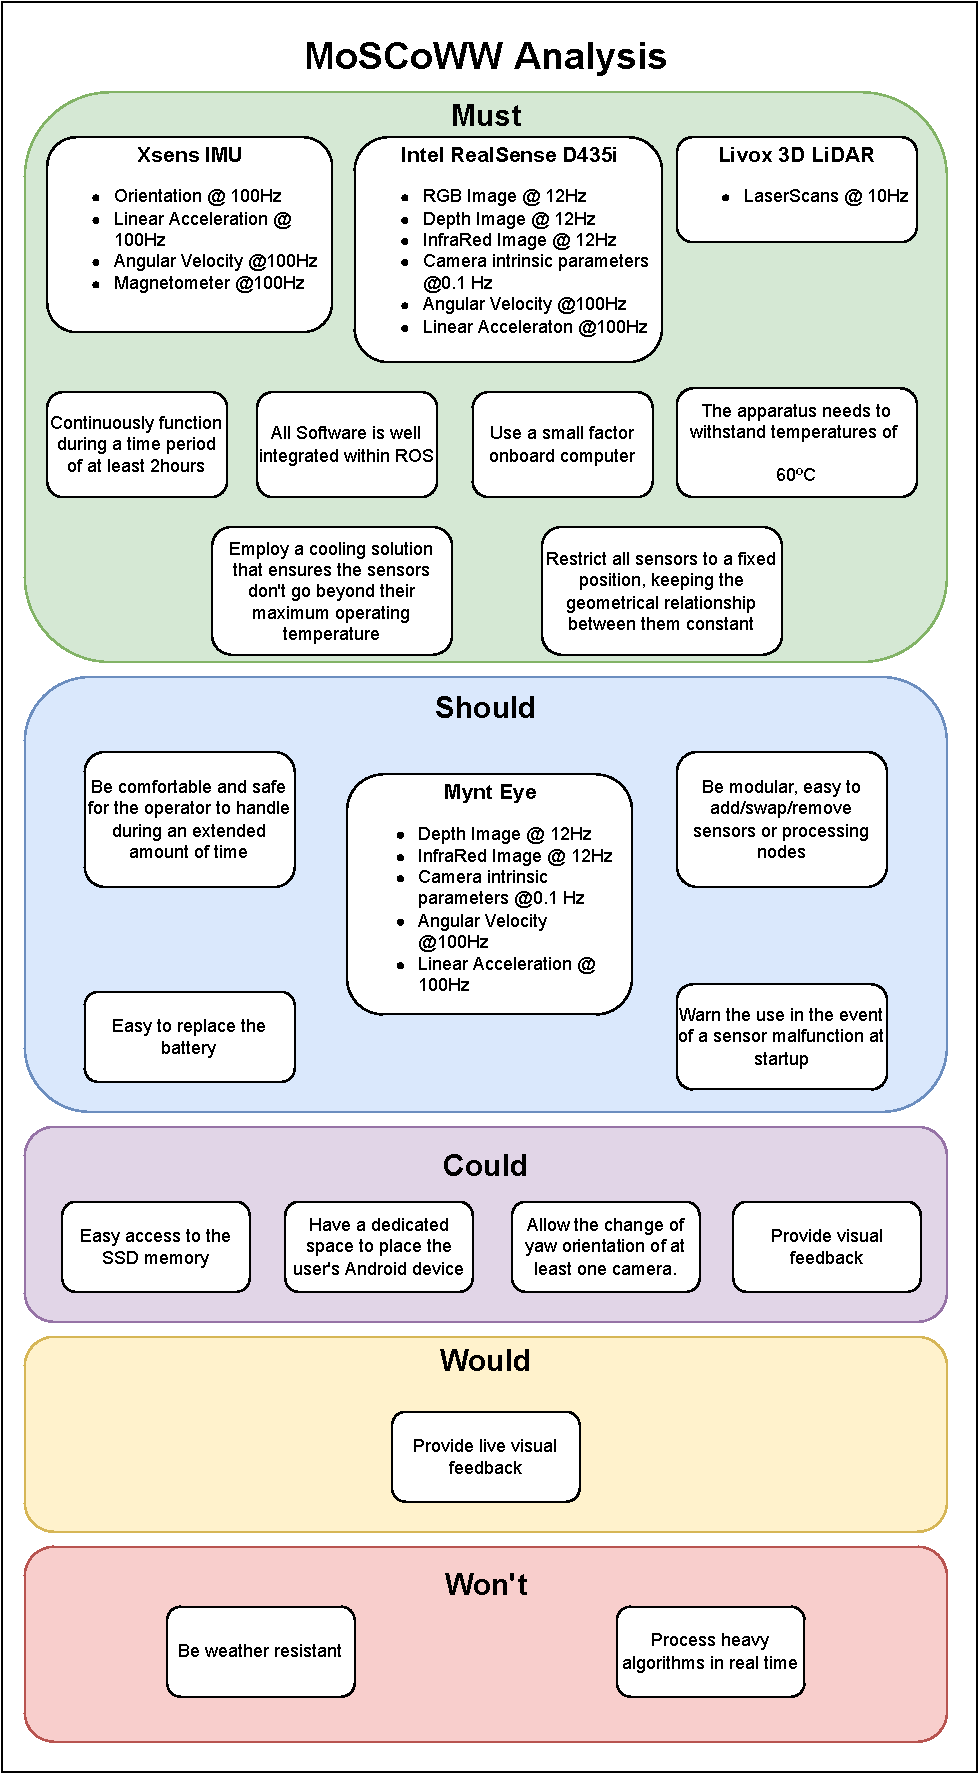
\includegraphics[width=0.65\linewidth]{images/introduction/moscoww_analysis.pdf}
    \caption{MoSCoWW analysis for the project}
    \label{fig: moscoww}
\end{figure}

\section{Dissertation Structure}
The document is structured as follows. In Section \ref*{chap:background}, essential concepts are explained while also displaying other works similar to the one presented here. A detailed description of the design and implementation of this project can be found in Chapter 3. In this chapter the overview of materials and the rationale for the decisions made are explained. The different steps required to implement a complete system are also discussed in Chapter 3. Chapter 4 examines the system's performance in several environments. In the last Chapter, a summary of how successful the project was is drawn, and suggestions for improvement are offered.